\subsection{Psykolog Nords problemstilling}

Psykolog Nord bruger to informationssystemer til at understøtte deres forretnin
g, se figur \ref{forretning:isfml}.
Dinero bruges som deres regnskabsprogram til at lave og sende fakturaer til deres klienter.

TerapeutBooking er deres nuværende bookingsystem.
Som det kan ses på figur \ref{forretning:isfml} understøttes virksomheden meget af de to informationssystemer, og derfor er det vigtigt, at de fungerer godt for dem.

Psykolog Nord har dog problemer med TerapeutBooking:

\begin{itemize}
    \item TerapeutBooking kan ikke håndtere en bruger tilknyttet flere lokationer.
    Derfor har Katrine to forskellige kalendre: En for hendes klienter i Aarhus og en i Aalborg.
    Katrine skal altså manuelt gå ind og blokere hendes ene kalender, når den anden kalender bliver booket.
    
    \item TerapeutBooking kan ikke håndtere flere kalendre, der bruger de samme lokaler.
    Det betyder, at da Miriam og Katrine lige nu begge tilbyder samtaler i Aarhus og Aalborg, skal de manuelt gå ind og blokere aftaler i hinandens kalendre.
    Hvis Katrine har en aftale i Aalborg om mandagen klokken 10 til 11, skal hun altså gå ind i Miriams kalender og blokere den tid.
    
   \item 
\end{itemize}

\begin{figure}
    \caption{Informationssystemers understøttelse af FML}
    \centering
        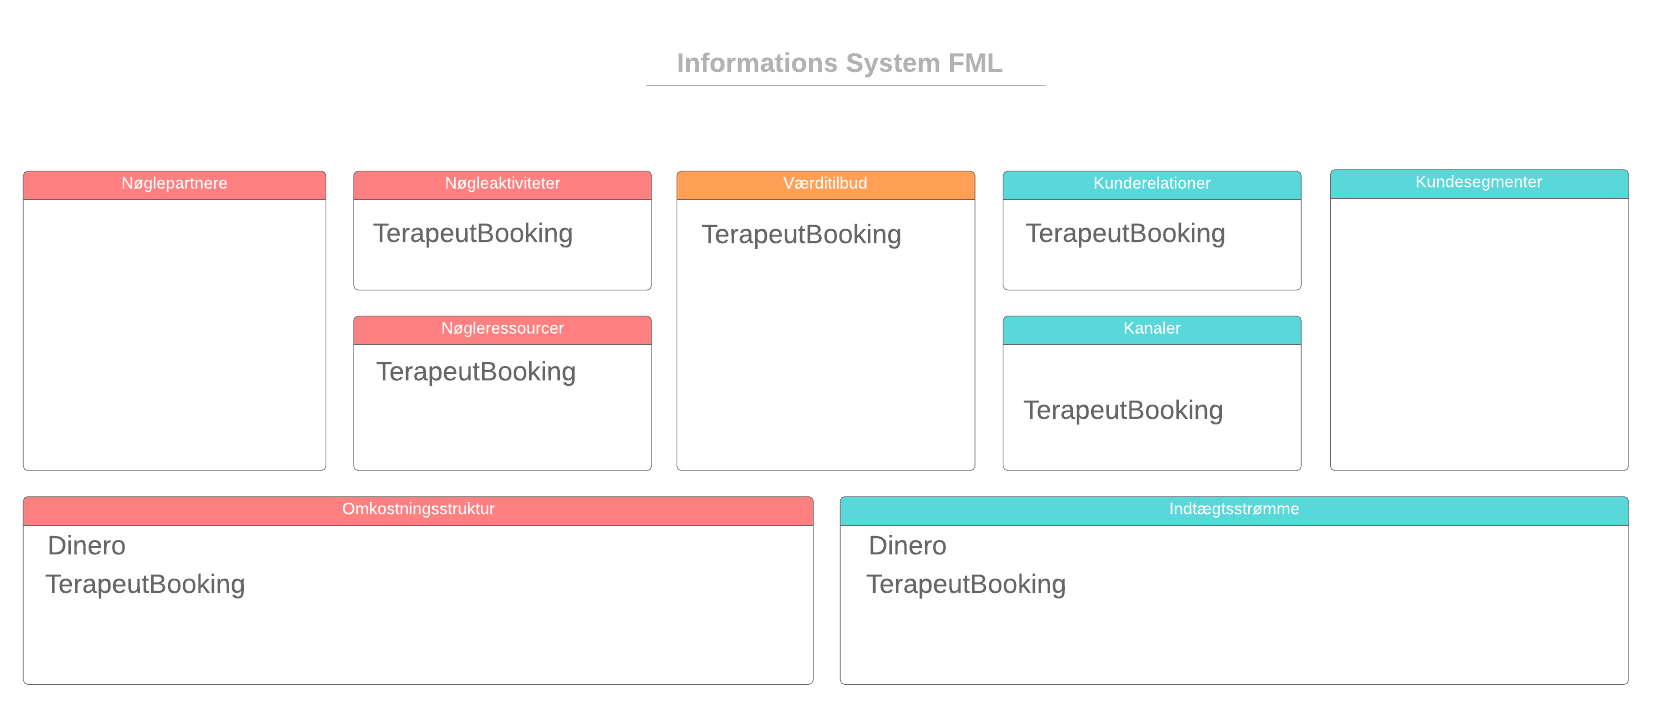
\includegraphics[scale=.5]{ISFML.png}
    \label{forretning:isfml}
\end{figure}